\section{Krylow-Verfahren für LGS}
\subsection{Grundlagen, Arnoldi}

\begin{karte}{Krylow-Raum}
    Zu \( A\in \C^{n,n} \) und \(b\in \C^n, b\neq 0 \), 
    heißt 
    \[ \Kcal_m(A,b) = \spann\set{b, Ab, \ldots, A^{m-1}b} \]
    der \(m\)-te \textit{Krylow-Raum} bezüglich \(A\) und \(b\).
\end{karte}

\begin{karte}{Konstruktion Krylow-Raum}
    Ist \(V_j \in \C^{n,j}\) eine Basis für \( \Kcal_j \) für \(j = 1,\ldots, m+1\), 
    wobei \( V_j = [V_{j-1} v_j] \), dann gibt es eine eindeutig bestimmte 
    nicht reduzierte obere Hessenbergmatrix \( \tilde{H}_m = (h_{ij}) \in \C^{m+1,m} \), 
    sodass 
    \[ A V_m = V_{m+1} \tilde{H}_m. \]
\end{karte}

\begin{karte}{Arnoldi-Algorithmus}
    \begin{tabbing}
        Zu gegebenem \(A\in \C^{n,n}, b\in \C^n\), berechne \( \beta = ||b||>0 \) \\
        \(v_1 = b/\beta\) \\
        for \= \( m = 1,2,\ldots \) do \\
        \> for \= \(j = 1,\ldots, m \) do \\
        \> \> \( h_{j,m} = v_j^H A v_m \) \\
        \> end for \\
        \> \( \tilde{v}_{m+1} = A v_m - \sum_{j=1}^m h_{j,m} v_j \) \\
        \> \( h_{m+1,m} = ||\tilde{v}_{m+1}|| \) \\
        \> \( v_{m+1} = \tilde{v}_{m+1}/h_{m+1,m} \) \\
        end for
    \end{tabbing}
    Unterschied zwischen Arnoldi und Gram-Schmidt: im \(m\)-ten Schritt wird
    nicht \( A^m b\) sondern \(A v_m\) verwendet. Dies ist mathematisch äquivalent, 
    allerdings aus Stabilitätsgründen zu bevorzugen.
\end{karte}

\begin{karte}{Eigenschaften Arnoldi-Verfahren}
    Seien \(V_m\) und \( \tilde{H}_m \) die Matrizen aus dem Arnoldi-Verfahren. 
    Dann gilt 
    \begin{enumerate}
        \item \( V_m^H V_m = I_m \),
        \item \( A V_m = V_{m+1} \tilde{H}_m = V_m H_m + h_{m+1,m} v_{m+1} e_m^T \),
        \item \( V_m^H A V_m = H_m \),
        \item \( V_{m+1}^H A V_m = \tilde{H}_m \),
        \item Für \( A = A^H \) ist \( H_m = H_m^H \) tridiagonal.
    \end{enumerate}
    \begin{tabular}{|c|c|c|}
        \hline
        Berechnung von & \(A\) beliebig & \(A\) hermitesch \\
        \hline
        \(A v_m\) & \(1\) Matrix-Vektormult. & \(1\) Matrix-Vektormult. \\
        \( h_{j,m} \) & \(m\) Skalarprodukte & \(1\) Skalarprodukt (\(h_{m-1,m} = \overline{h_{m,m-1}}\)) \\
        \( \tilde{v}_{m+1} \) & \(m\) \textsc{SAXPYs} & \(2\) \textsc{SAXPYs} \\
        \( h_{m+1,m} \) & \(1\) Skalarprodukt & \(1\) Skalarprodukt \\
        \( v_{m+1} \) & \(n\) Divisionen & \(n\) Divisionen \\\hline
        Speicher & \(m+1\) Vektoren & \(3\) Vektoren\\
        \hline
    \end{tabular}
\end{karte}

\begin{karte}{Abbruch Arnoldi-Prozess}
    Der Arnoldi-Algorithmus bricht ab, wenn \( h_{m+1,m} = 0 \) 
    bzw. \( A V_m = V_m H_m \) ist. Dann enthält der bisher konstruierte 
    Krylow-Raum bereits die exakte Lösung \( \widehat{x} = A^{-1}b \), d. h. 
    es existiert ein \( y_m \in \C^m \), sodass \( \widehat{x} = A^{-1}b = V_m y_m \).

    Beste Approximation: \(y_m\) soll Fehler \( f_m = \widehat{x} - x_m \)
    in einer gegebenen Norm \(||\cdot||\) minimieren: 
    \[ ||f_m|| = \min_{x\in \Kcal_m} ||\widehat{x} - x||. \]
\end{karte}

\begin{karte}{Residuenvektor}
    Sei \( r_m = A(\widehat{x} - x_m) \). 

    Es gilt \begin{align*}
        r_m &= b - A V_m y_m \\ 
        &= \beta v_1 - V_{m+1} \tilde{H}_m y_m \\
        &= V_{m+1} (\beta e_1 - \tilde{H}_m y_m).
    \end{align*}

    Also folgt 
    \[ ||r_m|| = ||V_{m+1}(\beta e_1 - \tilde{H}_m y_m)|| \leq ||V_{m+1}|| \;||\beta e_1 - \tilde{H}_m y_m||. \]
\end{karte}

\begin{karte}{Charakterisierung von \(y_m\)}
    (M): Minimiere \( ||\beta e_1 - \tilde{H}_m y|| \) über alle \(y \in \C^m\). 
    Dies führt auf ein lineares Ausgleichsproblem der Dimension \((m+1)\times m\). 
    \[ y_m = \beta (\tilde{H}_m^H \tilde{H}_m)^{-1} \tilde{H}_m^H e_1 = \beta \tilde{H}_m^+ e_1, \]
    wobei \( \tilde{H}_m^+ \) die Pseudoinverse von \( \tilde{H}_m \) bezeichnet.

    (G): Wähle \(y_m\) so, dass \(r_m\) orthogonal zu einem geeigneten Unterraum 
    \( \mathcal{W}_m \) der Dimension \(m\) ist. Für \( \mathcal{W}_m = \Kcal_m \)
    heißt die Bedingung \textit{Galerkin-Bedingung}, ansonsten \textit{Petrov-Galerkin-Bedingung}.
\end{karte}

\begin{karte}{(M) und (G) liefern eine Lösung}
    Ist \(A V_m = V_m H_m\) und ist \(W_m\) eine Basis von 
    \( \mathcal{W}_m \) mit \(W_m^H V_m\) nicht singulär, dann 
    ist \( x_m = V_m y_m \), wobei \(y_m\) durch (M) oder (G) charakterisiert ist, 
    die exakte Lösung, d. h. \( x_m = \widehat{x} = A^{-1}b \).

    Alle Krylov-Verfahren, deren Iterierte durch (M) oder (G) 
    bestimmt sind, liefern nach höchstens \(n\) Schritten die exakte Lösung.
\end{karte}

\subsection{Verfahren mit Arnoldi}

\begin{karte}{Residuenvektor Abschätzung}
    Ist \( V_{m+1} \) unitär und \(y_m = \beta \tilde{H}_m^+ e_1\) die Lösung 
    von (M), dann erfüllt \( x_m = V_m y_m \)
    \[ ||r_m|| = ||b - A x_m|| \leq ||b - Ax|| \quad \forall x\in \Kcal_m. \]
\end{karte}

\begin{karte}{GMRES}
    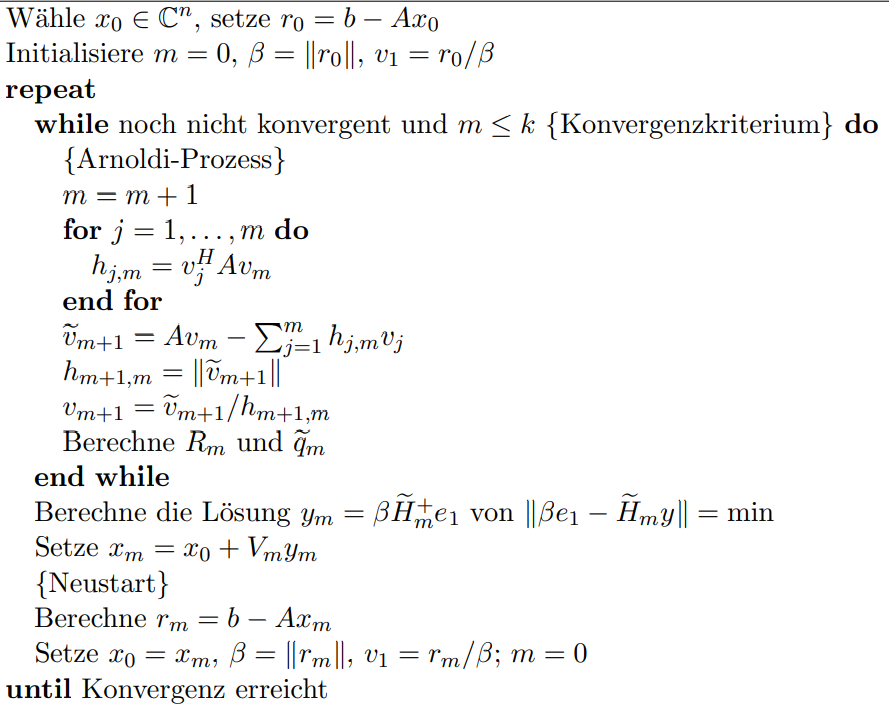
\includegraphics[width=0.8\textwidth]{GMRES.png}
\end{karte}

\begin{karte}{GMRES, FOM Eigenschaften}
    GMRES(\(k\)) wird nach \(k\) Iterationen neugestartet, falls der Speicherverbrauch 
    zu groß wird.
    Hierbei geht die Minimierungseigenschaft verloren und somit verlangsamt sich die Konvergenz.

    FOM ist die Galerkin-Bedingung kombiniert mit dem Arnoldi-Algorithmus. 
    Auch diese Variante kann neu gestartet werden.

    Sei \( V_{m+1} \) unitär und \( \mathcal{W}_m = \Kcal_m \). Dann 
    existiert eine Lösung von (G) genau dann, wenn \(H_m\) nicht singulär ist. 
    In diesem Fall ist \(x_m = V_m y_m\), wobei \(H_m y_m = \beta e_1\).
\end{karte}

\begin{karte}{Wertebereich \( H_m \)}
    Ist \(V_m\) unitär, dann gilt 
    \( \mathcal{F}(H_m) \subseteq \mathcal{F}(A) \). Insbesondere folgt aus
    \( 0 \notin \mathcal{F}(A) \), dass \( H_m \) für alle \(m\) nicht singulär ist.
\end{karte}

\begin{karte}{Wünschenswerte Eigenschaften eines Krylowverfahrens}
    Wünschenswert sind
    \begin{enumerate}
        \item Minimierung des Fehlers (oder Residuums) in einer festen Norm unabhängig vom Startwert
        \item kurze Rekursionen (gleicher Aufwand in jedem Schritt)
    \end{enumerate}

    Es ist i. A. nicht möglich, beides gleichzeitig zu erfüllen. 
    GMRES erfüllt 1., jedoch nicht 2., FOM erfüllt weder 1. noch 2..
    Das nichtsymmetrische Lanczos-Verfahren erfüllt 2. und 1. in einer abgeschwächten Form.
\end{karte}

\subsection{Nichtsymm. Lanczos-Verfahren}

\begin{karte}{Nichtsymmetrisches Lanczos-Verfahren Grundprinzip}
    Man berechnet eine Basis \( (v_j)_j \) von \( \Kcal_m(A,b) \)
    und eine Basis \( (w_j)_j \) von \( \Kcal_m(A^H, c) \) für einen geeigneten 
    Vektor \(c\in \C^n\). 

    Wir verlangen außerdem Biorthogonalität der beiden Basen:
    \[ w_j^H v_k = \begin{cases}
        0, & j\neq k, \\ \delta_k \neq 0, & j = k,
    \end{cases} \]
    oder 
    \[ v_m \bot \Kcal_{m-1}(A^H, c), \quad w_m \bot \Kcal_{m-1}(A, b). \]
\end{karte}

\begin{karte}{Nichtsymmetrisches Lanczos-Verfahren}
    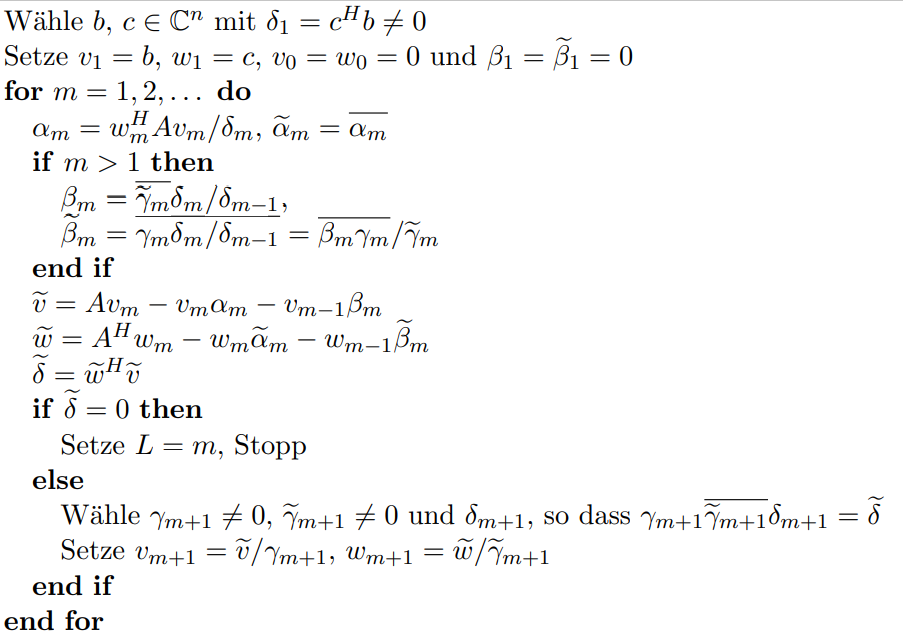
\includegraphics[width=0.8\textwidth]{Nichtsymmetrisches-Lanczos-Verfahren.png}
\end{karte}

\begin{karte}{Nichtsymmetrisches Lanczos-Verfahren Eigenschaften}
    Für das nichtsymmetrische Lanczos-Verfahren gilt 
    \begin{enumerate}
        \item \( W_m^H V_m = D_m = \diag(\delta_1, \ldots, \delta_m), m = 1,\ldots, L \),
        \item \( A V_m = V_{m+1} \tilde{T}_m = V_m T_m + \gamma_{m+1} v_{m+1} e_m^T \),
        \item \( A^H W_m = W_{m+1} \tilde{S}_m = W_m S_m + \tilde{\gamma}_{m+1} w_{m+1} e_m^T \), 
        wobei \(\tilde{S}_m\) analog zu \(\tilde{T}_m\) definiert ist, jedoch mit Koeffizienten 
        \( \tilde{\alpha}_j, \tilde{\beta}_j, \tilde{\gamma}_j \), 
        \item \( W_m^H A V_m = D_m T_m = S_m^H D_m \),
        \item in exakter Arithmetik bricht der Lanczos-Prozess nach \(m= L-1\) 
        Schritten ab, wobei 
        \[ 1 \leq L \leq \min\set{ \dim \Kcal_n(A,b), \dim \Kcal_n(A^H, c) }. \]
    \end{enumerate}
\end{karte}

\begin{karte}{Zusammenbruch}
    Der Lanczos-Algorithmus bricht ab, wenn 
    \( \tilde{\delta} = \tilde{w}_L^H \tilde{v}_L = 0 \). 
    Hierfür gibt es zwei verschiedene Ursachen:
    \begin{description}
        \item[Regulärer Zusammenbruch] \( \tilde{w}_L = 0 \) 
        oder \( \tilde{v}_L = 0\). Ist \( \tilde{w}_l = 0 \), 
        dann spannen die linken Lanczos-Vektoren einen \(A^H\)-invarianten 
        Unterraum auf, sonst spannen die rechten Lanczos-Vektoren einen 
        \(A\)-invarianten Unterraum auf.
        \item[Ernsthafter Zusammenbruch] \( \tilde{w}_l \neq 0 \neq \tilde{v}_L \). 
        Die Lanczos-Vektoren spannen weder einen \(A\)- noch einen \(A^H\)-invarianten 
        Unterraum auf.
    \end{description}
\end{karte}

\subsection{Konjugierte Gradienten}

\begin{karte}{}

\end{karte}

\begin{karte}{}

\end{karte}

\begin{karte}{}

\end{karte}

\begin{karte}{}

\end{karte}